\documentclass[a4paper, 14pt]{extarticle}

\usepackage[T2A]{fontenc}
\usepackage{natbib}
\usepackage{graphicx}
\usepackage[english, russian]{babel}
\usepackage{fontspec}
\usepackage{amsmath}
\usepackage{amsfonts}
\usepackage{amssymb}
\usepackage{amsthm}
\usepackage{mathtools}
\usepackage{mathrsfs}
\usepackage{icomma}
\usepackage{fullpage}
\usepackage{ulem}
\usepackage{setspace}
\usepackage{listings}
\usepackage{indentfirst}
\usepackage[left=2cm,right=1.5cm,top=2cm,bottom=2cm]{geometry}
\usepackage{xcolor}
\usepackage{float}
\usepackage{csquotes}
\usepackage{hyperref}
\usepackage{graphics}



\definecolor{urlcolor}{HTML}{0000FF} % цвет гиперссылок
\definecolor{linkcolor}{HTML}{000000} % цвет гиперссылок
\hypersetup{pdfstartview=FitH, linkcolor=linkcolor, urlcolor=urlcolor, colorlinks=true}


\setmainfont{Times New Roman}
\setlength{\parindent}{5ex}
\setlength{\parskip}{1em}
\renewcommand{\baselinestretch}{1}

\graphicspath{{images/}}


\definecolor{buzzlightyear}{HTML}{8757A5}
\definecolor{grass}{HTML}{738D06}
\definecolor{literal}{HTML}{F18A2B}
\definecolor{commentcolor}{HTML}{8E908B}

\lstdefinestyle{habrstyle}{
    backgroundcolor=\color{white},
    commentstyle=\color{commentcolor},
    keywordstyle=\bfseries\color{buzzlightyear},
    numberstyle=\tiny\color{commentcolor},
    stringstyle=\color{grass},
    basicstyle=\ttfamily\footnotesize,
    breakatwhitespace=false,
    breaklines=true,
    captionpos=b,
    keepspaces=true,
    numbers=left,
    numbersep=5pt,
    showspaces=false,
    showstringspaces=false,
    showtabs=false,
    tabsize=4
}

\lstset{style=habrstyle}

\begin{document}
    % НАЧАЛО ТИТУЛЬНОГО ЛИСТА
    \begin{center}
        \begin{center}
            \hfill \break
            \normalsize{Санкт-Петербургский государственный политехнический}\\
            \normalsize{университет Петра Великого}\\
            \hfill \break
            \normalsize{\textbf{Высшая школа интеллектуальных систем и}}\\
            \normalsize{\textbf{суперкомпьютерных технологий}}\\
            \hfill \break
            \hfill \break
            \hfill \break
            \normalsize{Лабораторная работа}\\
            \hfill \break
            \normalsize{\LARGE Дискретное косинусное преобразование}\\
        \end{center}
        \hfill \break
        \hfill \break
        \hfill \break
        \hfill \break
        \hfill \break
        \hfill \break
        \hfill \break
        \hfill \break
        \hfill \break
        \hfill \break
        \begin{tabbing}
            Выполнил студент гр. 3530901/80201 \`И.С. Иванов\\
            \\
            Преподаватель: \`Н.В. Богач\\
        \end{tabbing}
        \hfill \break
        \hfill \break
        \hfill \break
        \hfill \break
        \begin{center}
            Санкт-Петербург\\
            2021
        \end{center}
        \thispagestyle{empty}
    \end{center}
    % КОНЕЦ ТИТУЛЬНОГО ЛИСТА

    % ОГЛАВЛЕНИЕ
    \newpage
    \tableofcontents

    % СПИСОК ИЛЛЮСТРАЦИЙ
    \newpage
    \listoffigures

    % СПИСОК ЛИСТИНГОВ
    \newpage
    \lstlistoflistings

    \newpage


    \section{Упражнение №1}
    \label{sec:1}

    В первом упражнении необходимо проверить, что \texttt{analyze1} требует времени пропорционально \texttt{\(n^3\)}, а \texttt{analyze2} пропорционально \texttt{\(n^2\)} путем запуска их с несколькими разными массивами.
    Для этого необходимо воспользоваться \texttt{timeint}.

    Необходимо создать сигнал на основе некоррелируемого гауссовского шума

    \begin{lstlisting}[language=Python, caption= Создание сигнал на основе некоррелируемого гауссовского шума, label={lst:make_signal}]
        from thinkdsp import UncorrelatedGaussianNoise

        signal = UncorrelatedGaussianNoise()
        noise = signal.make_wave(duration=1.0, framerate=16384)
        noise.ys.shape
    \end{lstlisting}

    Создадим функция, которая будет брать и отображать массив результатов, а так же выстраивать их в прямую линию

    \begin{lstlisting}[language=Python, caption=Функция plot\_bests, label={lst:plot_bests}]
        from scipy.stats import linregress

        loglog = dict(xscale='log', yscale='log')

        def plot_bests(ns, bests):
            plt.plot(ns, bests)
            decorate(**loglog)

            x = np.log(ns)
            y = np.log(bests)
            t = linregress(x,y)
            slope = t[0]

            return slope
    \end{lstlisting}

    Создадим функция \texttt{analyze1}

    \begin{lstlisting}[language=Python, caption= Функция analyze1, label={lst:analyze1}]
        PI2 = np.pi * 2

        def analyze1(ys, fs, ts):
            args = np.outer(ts, fs)
            M = np.cos(PI2 * args)
            amps = np.linalg.solve(M, ys)
            return amps
    \end{lstlisting}

    Создадим тестовые данные.

    \begin{lstlisting}[language=Python, caption= Создание тестовых данных, label={lst:make_test_data}]
        ns = 2 ** np.arange(6, 13)
    \end{lstlisting}

    Далее используем данную функцию.

    \begin{lstlisting}[language=Python, caption= Тестирование функции, label={lst:test_analyze1}]
        results = []
        for N in ns:
            print(N)
            ts = (0.5 + np.arange(N)) / N
            freqs = (0.5 + np.arange(N)) / 2
            ys = noise.ys[:N]
            result = %timeit -r1 -o func(ys, freqs, ts)
            results.append(result)

        bests = [result.best for result in results]

        plot_bests(ns, bests)
    \end{lstlisting}

    \begin{lstlisting}[language=Python, caption= Получившиеся данные, label={lst:data_1}]
        64
        94 µs ± 0 ns per loop (mean ± std. dev. of 1 run, 10000 loops each)
        128
        260 µs ± 0 ns per loop (mean ± std. dev. of 1 run, 1000 loops each)
        256
        2.18 ms ± 0 ns per loop (mean ± std. dev. of 1 run, 100 loops each)
        512
        8.18 ms ± 0 ns per loop (mean ± std. dev. of 1 run, 100 loops each)
        1024
        36.6 ms ± 0 ns per loop (mean ± std. dev. of 1 run, 10 loops each)
        2048
        183 ms ± 0 ns per loop (mean ± std. dev. of 1 run, 10 loops each)
        4096
        770 ms ± 0 ns per loop (mean ± std. dev. of 1 run, 1 loop each)

        2.2137508528116374
    \end{lstlisting}

    \begin{figure}[H]
        \centering
        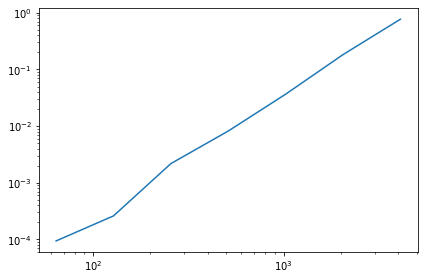
\includegraphics[width=0.8\linewidth]{analyze_1_wave}
        \caption{Получившийся график}
        \label{fig:analyze_1_wave}
    \end{figure}

    Создадим функцию \texttt{analyze2}.

    \begin{lstlisting}[language=Python, caption= Функция analyze2, label={lst:analyze2}]
        def analyze2(ys, fs, ts):
            args = np.outer(ts, fs)
            M = np.cos(PI2 * args)
            amps = np.dot(M, ys) / 2
            return amps
    \end{lstlisting}

    \begin{lstlisting}[language=Python, caption= Получившиеся данные, label={lst:data_2}]
        64
        45 µs ± 0 ns per loop (mean ± std. dev. of 1 run, 10000 loops each)
        128
        204 µs ± 0 ns per loop (mean ± std. dev. of 1 run, 1000 loops each)
        256
        1.35 ms ± 0 ns per loop (mean ± std. dev. of 1 run, 1000 loops each)
        512
        4.19 ms ± 0 ns per loop (mean ± std. dev. of 1 run, 100 loops each)
        1024
        18.9 ms ± 0 ns per loop (mean ± std. dev. of 1 run, 100 loops each)
        2048
        78.1 ms ± 0 ns per loop (mean ± std. dev. of 1 run, 10 loops each)
        4096
        261 ms ± 0 ns per loop (mean ± std. dev. of 1 run, 1 loop each)

        2.088196535313128
    \end{lstlisting}

    \begin{figure}[H]
        \centering
        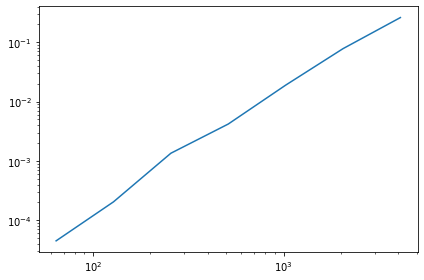
\includegraphics[width=0.8\linewidth]{analyze_2_wave}
        \caption{Получившийся график}
        \label{fig:analyze_2_wave}
    \end{figure}

    Отобразим два графика на одном для сравнения.

    \begin{figure}[H]
        \centering
        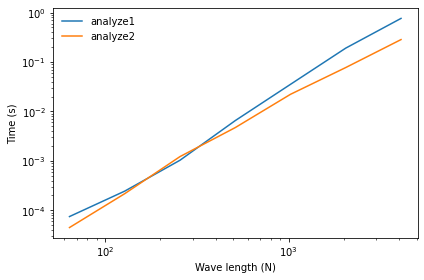
\includegraphics[width=0.8\linewidth]{analyze_1_2_wave}
        \caption{Совмещенный график}
        \label{fig:analyze_1_2_wave}
    \end{figure}


    \newpage


    \section{Упражнение №2}
    \label{sec:2}

    Во втором упражнении необходимо реализовать версию алгоритма "DCT" для сжатия звука

    Скачаем звук с сайта \href{https://freesound.org}{freesound.org}.
    Прочитаем его.
    Выделим сегмент длительностью 0.5 секунд.

    Далее выведем график "DCT"

    \begin{figure}[H]
        \centering
        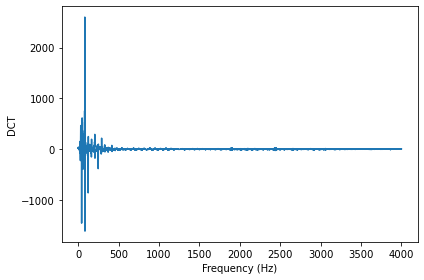
\includegraphics[width=0.8\linewidth]{bass_dct}
        \caption{График DCT сегмента}
        \label{fig:bass_dct}
    \end{figure}

    На графике видно, что в сегменте много точек с нулевой амплитудой.
    Напишем функцию \texttt{compress} для обнуления элементов ниже порога \texttt{thresh}.

    \begin{lstlisting}[language=Python, caption= Функция compress, label={lst:compress}]
        def compress(dct, thresh=1):
            count = 0
            for i, amp in enumerate(dct.amps):
                if np.abs(amp) < thresh:
                    dct.hs[i] = 0
                    count += 1

            n = len(dct.amps)
            print(count, n, 100 * count / n, sep='\t')
    \end{lstlisting}

    Применим функцию к выделенному сегменту.

    \begin{figure}[H]
        \centering
        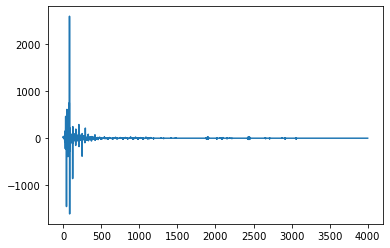
\includegraphics[width=0.8\linewidth]{segment_after_dct}
        \caption{График сегмента после DCT}
        \label{fig:segment_after_dct}
    \end{figure}

    Графики почти не отличаются.
    При прослушивании результата, изменения почти не различимы.

    Для сжатия более длинного фрагмента необходимо написать функцию \texttt{make\_dct\_spectrogram}.

    \begin{lstlisting}[language=Python, caption= Функция make\_dct\_spectrogram, label={lst:make_dct_spectrogram}]
        from thinkdsp import Spectrogram

        def make_dct_spectrogram(wave, seg_length):
            window = np.hamming(seg_length)
            i, j = 0, seg_length
            step = seg_length // 2
            spec_map = {}

            while j < len(wave.ys):
                segment = wave.slice(i, j)
                segment.window(window)
                t = (segment.start + segment.end) / 2
                spec_map[t] = segment.make_dct()

                i += step
                j += step

            return Spectrogram(spec_map, seg_length)
    \end{lstlisting}

    Теперь необходимо создать спектрограмму "DCT" с помощью только что созданной функции и применить \texttt{compress} для каждого сегмента.

    \begin{lstlisting}[language=Python, caption= Применение "DCT" для всего файла, label={lst:dct_to_spectrogram}]
        spectro = make_dct_spectrogram(wave, seg_length=1024)
        for t, dct in sorted(spectro.spec_map.items()):
            compress(dct, thresh=0.2)
    \end{lstlisting}

    \begin{lstlisting}[language=Python, caption= Пример вывода функции label={lst:example_output}]
        999	1024	97.55859375
        1004	1024	98.046875
        1014	1024	99.0234375
        1011	1024	98.73046875
        1010	1024	98.6328125
        1012	1024	98.828125
        1012	1024	98.828125
        778	1024	75.9765625
        540	1024	52.734375
        527	1024	51.46484375
        555	1024	54.19921875
        568	1024	55.46875
        588	1024	57.421875
        647	1024	63.18359375
        689	1024	67.28515625
        708	1024	69.140625
        767	1024	74.90234375
        824	1024	80.46875
        919	1024	89.74609375
        951	1024	92.87109375
    \end{lstlisting}

    Прослушав получившийся сигнал и исходный, никаких изменений не слышно.
    Управление параметром \texttt{thresh} влияет на получаемый после сжатия шум.

    \newpage


    \section{Упражнение №3}
    \label{sec:3}

    В третьем упражнении нам необходимо запустить файл \texttt{phase.ipynb}, пройтись по всем примерам, после выбрать другой сегмент исходного аудио файла и провести с ним те же манипуляции.

    Для проведения действий из файла необходимо взять функции \texttt{plot\_angle} и \texttt{plot\_three}.

    \begin{lstlisting}[language=Python, caption= Функция plot\_angle, label={lst:plot_angle}]
        def plot_angle(spectrum, thresh=1):
            angles = spectrum.angles
            angles[spectrum.amps < thresh] = np.nan
            plt.plot(spectrum.fs, angles, 'x')
            decorate(xlabel='Frequency (Hz)',
                     ylabel='Phase (radian)')
    \end{lstlisting}

    \begin{lstlisting}[language=Python, caption= Функция plot\_three, label={lst:plot_three}]
        def plot_three(spectrum, thresh=1):
            plt.figure(figsize=(10, 4))
            plt.subplot(1,3,1)
            spectrum.plot()
            plt.subplot(1,3,2)
            plot_angle(spectrum, thresh=thresh)
            plt.subplot(1,3,3)
            wave = spectrum.make_wave()
            wave.unbias()
            wave.normalize()
            wave.segment(duration=0.01).plot()
            wave.make_audio()
    \end{lstlisting}

    Возьмем фрагмент длительностью 1 секундой, начиная с 5 секунды.
    Вычислим его спектр и вызовем функцию \texttt{plot\_three}.

    \begin{figure}[H]
        \centering
        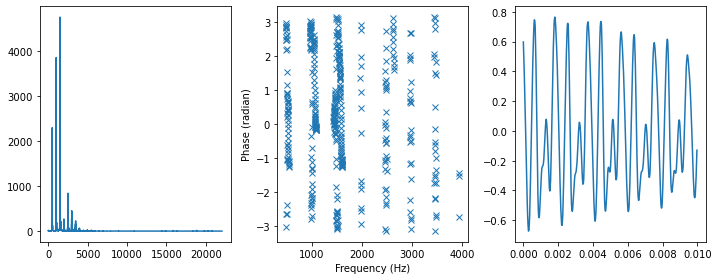
\includegraphics[width=0.8\linewidth]{oboe_spectrum_plot_three}
        \caption{График спектра}
        \label{fig:oboe_spectrum_plot_three}
    \end{figure}

    Добавим функцию \texttt{zero\_angle}, выдающая результат, в котором \texttt{angle} = 0.

    \begin{lstlisting}[language=Python, caption= Функция zero\_angle, label={lst:zero_angle}]
        def zero_angle(spectrum):
            res = spectrum.copy()
            res.hs = res.amps
            return res
    \end{lstlisting}

    Получим спектр с помощью \texttt{zero\_angle} и выведем графики с помощью \texttt{plot\_three}.

    \begin{figure}[H]
        \centering
        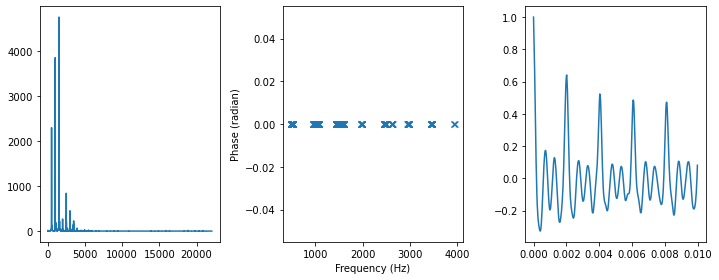
\includegraphics[width=0.8\linewidth]{oboe_zero_angle}
        \caption{Графики полученные с помощью zero\_angle и plot\_three}
        \label{fig:oboe_zero_angle}
    \end{figure}

    Добавим функцию \texttt{rotate\_angle}, выдающая результат, в котором \texttt{angle} изменен на 1 радиан.

    \begin{lstlisting}[language=Python, caption= Функция rotate\_angle, label={lst:rotate_angle}]
        def rotate_angle(spectrum, offset):
            res = spectrum.copy()
            res.hs *= np.exp(1j * offset)
            return res
    \end{lstlisting}

    Получим спектр с помощью \texttt{rotate\_angle} и выведем графики с помощью \texttt{plot\_three}.

    \begin{figure}[H]
        \centering
        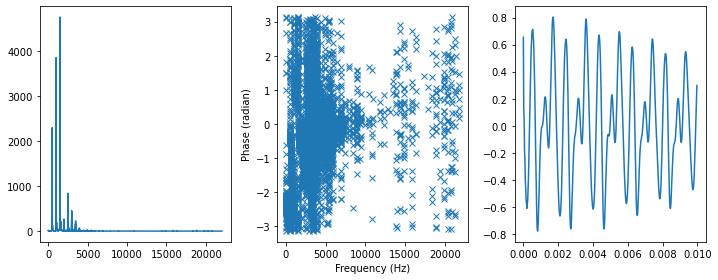
\includegraphics[width=0.8\linewidth]{oboe_rotate_angle}
        \caption{Графики полученные с помощью rotate\_angle и plot\_three}
        \label{fig:oboe_rotate_angle}
    \end{figure}

    Добавим функцию \texttt{random\_angle}, выдающая результат, в котором \texttt{angle} имеет случайное значение.

    \begin{lstlisting}[language=Python, caption= Функция random\_angle, label={lst:random_angle}]
        PI2 = np.pi * 2

        def random_angle(spectrum):
            res = spectrum.copy()
            angles = np.random.uniform(0, PI2, len(spectrum))
            res.hs *= np.exp(1j * angles)
            return res
    \end{lstlisting}

    Получим спектр с помощью \texttt{random\_angle} и выведем графики с помощью \texttt{plot\_three}.

    \begin{figure}[H]
        \centering
        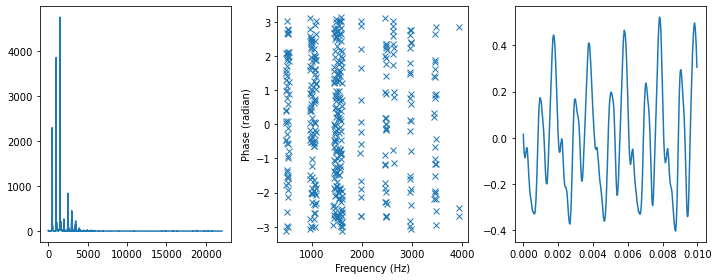
\includegraphics[width=0.8\linewidth]{oboe_random_angle}
        \caption{Графики полученные с помощью random\_angle и plot\_three}
        \label{fig:oboe_random_angle}
    \end{figure}

    Из полученных результатов можно сделать вывод, что при рандомизация немного приглушила звук, а установка \texttt{angle} в ноль искажает звук.

    \newpage



    \section{Выводы}
    \label{sec:conclusions}

    В результате выполнения данной лабораторной работы мы изучили, понятие DCT.
    Были проверены функции \texttt{analyze1} и \texttt{analyze2}.
    Была создана функция \texttt{make\_dct\_spectrogram} для сжатия звуковой дорожки.
    Было изучено понятие \texttt{angle} и закреплено его влияние на практике.

\end{document}